% Tutto quello riguardante il progetto andrà in questo capitolo 

\chapter{Tecnologie utilizzate}\label{chap:tec}

\postit{Ho visto che solo nell'ultimo hai messo dei vantaggi. Se hai voglia potresti schematizzarne dappertutto come anche elencare degli aspetti negativi dell'utilizzo}

\section{Ambiente di sviluppo}
\subsection{Docker}
	\begin{figure}[H] 
		\centering
		
\includegraphics[scale=0.3]{docker}
		\caption{Logo Docker}
	\end{figure}
Docker permette di automatizzare lo sviluppo di applicazione dentro a 
determinati container software, 
in modo da fornire una virtualizzazione a livello del sistema operativo Linux
senza che sia necessario istanziare delle macchine virtuali pienamente 
operative.
\note{Non mi piace molto come frase. Metterei tipo \emph{Docker è una
piattaforma per lo sviluppo, rilascio e esecuzione di applicazioni software
all'interno di container. Quest'ultimi forniscono un'astrazione dall'ambiente in
cui vengono utilizzati, sfruttando la virtualizzazione del sistema Linux. Tutto
ciò è possibile evitando la creazione di macchine virtuali.} Se aggiungere
cose, tipo cosa sono i container potresti prendere da qui
https://docs.docker.com/get-started/\#docker-concepts come ho fatto anche io}
I container sono assimilabili a delle macchine virtuali modulari con la
peculiarità di essere molto leggere: in questo modo risulta più facile creare,
distribuire, copiare e spostare i container da un ambiente all'altro.
Ogni container è un processo isolato dagli altri \mmh{container}{ripetizione
ma non mi viene come cambiare la frase} e dal sistema ospite stesso: ogni
volta che viene mandato in esecuzione si avrà un ambiente pulito, con le
caratteristiche desiderate. \note{Qui volevi dire che se crei un
nuovo container è tutto nuovo vero? In caso metterei qualcosa di simile
\emph{ogni volta che viene istanziato un nuovo container si avrà un ambiente
\emph{pulito}, ovvero nuovo e indipendente da container precedentemente creati,
e con le caratteristiche specificate.}} 
Per sviluppare l'applicazione Teamwork è stato utilizzato Docker 18.03
Community Edition per Ubuntu Bionic. In questo modo si è potuto
\mmh{caricare}{ripetizione, va bene \emph{distribuire}?} nelle macchine locali
un container di Zimbra e del core Zextras con la zimlet OpenChat caricata così
da sviluppare l'applicativo in un ambiente sicuro e pulito.

\subsection{IntelliJ IDEA} \label{subsec:IntelliJ}
	\begin{figure}[H] 
		\centering
		
\includegraphics[scale=0.2]{intellij-idea}
		\caption{Logo IntelliJ IDEA}
	\end{figure}
IntelliJ IDEA è un Integrated Development Environment (IDE) multi-linguaggio e 
multi-piattaforma. 
È stata utilizzata la \mmh{versione}{solitamente si parla di \emph{edition}} Ultimate in quanto era necessario un editor che 
supportasse  
JavaScript/TypeScript, mentre la Community version non supporta questi 
linguaggi. 
Dovendo creare un'applicazione con numerose referenze al codice della zimlet 
OpenChat e di Zimbra 
sono state sfruttate al meglio le funzionalità per analizzare il codice e 
comprendere le 
dipendenze esistenti.

\subsection{Expo} \label{subsec:expo}
	\begin{figure}[H] 
		\centering
		
\includegraphics[scale=0.05]{expo}
		\caption{Logo Expo}
	\end{figure}
Expo è una toolchain open source che permette la gestione di un progetto React 
Native utilizzando l'SDK di Expo. L'SDK Expo è una libreria nativa e JavaScript 
che fornisce l'accesso alle funzionalità del sistema del dispositivo (come la 
fotocamera, i contatti, la memoria locale) senza il bisogno di utilizzare xCode 
o Android Studio, né di utilizzare codice nativo. Fornisce l'accesso a servizi 
che in genere sono difficili da gestire nativamente, ma sono richiesti da quasi 
tutte le app come le notifiche push o creare binari nativi pronti per la 
distribuzione nell'app store.
Inoltre risulta molto facile lo sviluppo e il test dato che permette delle 
build automatiche nei loro server che possono eseguire in real-time il codice 
sia in simulatori che in dispositivi mobili.


\section{Linguaggi, librerie e strumenti di programmazione}

\subsection{React Native}
\begin{figure}[H] 
	\centering
	
\includegraphics[scale=0.1]{React}
	\caption{Logo React Native}
\end{figure}
React Native è un framework per lo sviluppo di applicazioni mobile in
JavaScript, \mmh{destinate a piattaforme native}{Non ho capito}. Questo permette di 
unificare l'esperienza di sviluppo su diversi sistemi operativi. Infatti React 
Native utilizza gli stessi \mmh{blocchi fondamentali}{o lasci \emph{building blocks} oppure metterei \emph{le stesse componenti}} dell'interfaccia utente che 
vengono utilizzate da app native iOS e Android. \note{toglierei \emph{sviluppate utilizzando i linguaggi Swift e Java} per evitare le ripetizioni con la frase dopo}
Si possono comunque integrare dei componenti scritti in Objective-C,
Java o Swift così da passare al codice nativo nel caso fosse necessario
ottimizzare alcuni aspetti dell'applicazione in base alla piattaforma.
React Native si basa su ReactJS nel quale è fondamentale il concetto di
componente. Un componente è \mmh{qualcosa}{\emph{oggetto} è troppo ambiguo? sennò lascia \emph{qualcosa}} che ha uno stato, che può accettare
delle proprietà e che ha un proprio ciclo di vita. Questo approccio di
sviluppo atomico risulta perfetto per effettuare Unit Test o per creare
componenti più complessi includendone altri più semplici.

\subsection{TypeScript}
\begin{figure}[H] 
	\centering
	
\includegraphics[scale=0.07]{ts}
	\caption{Logo TypeScript}
\end{figure}
TypeScript è un linguaggio di programmazione sviluppato da Microsoft che
estende la sintassi di JavaScript. È nato per poter utilizzare le funzionalità
di JavaScript per lo sviluppo di grandi applicazioni, in quanto ne aumenta la
sicurezza e la robustezza del codice tramite l'aggiunta di classi,
interfacce, moduli, tipizzazione e altre funzionalità importanti per la 
comprensione di un grande progetto.
Il codice TypeScript sviluppato viene ricompilato in JavaScript per poter
essere interpretato da browser o app.

\subsection{TSLint}
\begin{figure}[H] 
	\centering
	
\includegraphics[scale=0.4]{TSlint}
	\caption{Logo TS Lint}
\end{figure}
TSLint è uno strumento di analisi statica per il codice scritto in TypeScript che offre funzionalità estendibili e personalizzabili per la leggibilità, la manutenibilità e gli errori di funzionalità. È supportato da molti dei moderni editor, compreso IntelliJ IDEA (sez. \ref{subsec:IntelliJ}), utilizzato per il progetto.

\subsection{Redux}
\begin{figure}[H] 
	\centering
	
\includegraphics[scale=0.06]{redux}
	\caption{Logo Redux}
\end{figure}
Redux è una libreria Javascript per la gestione semplificata dello stato delle applicazioni web. In ReactJS e React Native ogni componente possiede uno stato che può cambiare durante il suo ciclo di vita. Questo stato è interno ad ogni singola componente ed è difficile, a volte impossibile, la comunicazione di questi dati tra componenti diverse.
Redux, invece, permette la creazione di uno stato condiviso, utilizzato da ogni
componente. In tal modo, è possibile sincronizzare le modifiche e quindi avere
dei dati coerenti  tra i vari componenti, avendo così dati coerenti nelle varie
componenti.
Redux è stato implementato basandosi su una particolare architettura:
\hyperref[subsubsec:flux]{Flux}.

\subsubsection{Flux}\label{subsubsec:flux}
 Flux è un pattern architetturale che ha ispirato Redux, utilizzato per la creazione di \mmh{applicazioni web lato client}{troppo traduzione 1 a 1 dall'inglese. Io lascerei \emph{client-side} e piuttosto metterei nel glossario qualcosa che spiega di applicazioni la cui parte dinamica viene eseguita sul client}. Esso utilizza un flusso di dati unidirezionale per gestire al meglio la sincronizzazione degli stati tra le componenti React. In questo modo si è sicuri che lo stato dello store sia sempre uguale in tutte le componenti che compongono la view.
 \begin{figure}[H] 
 	\centering
 	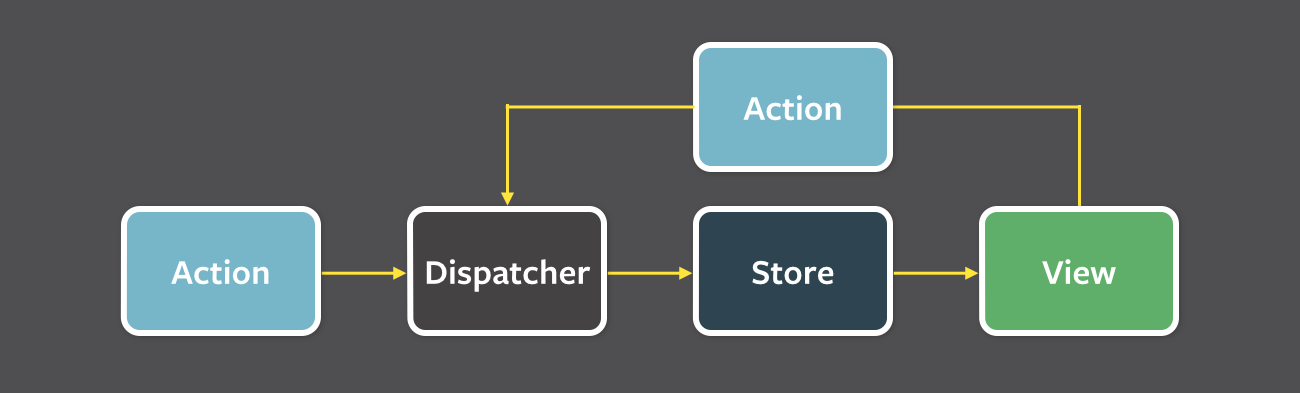
\includegraphics[scale=0.3]{flux}
 	\caption{Flusso dei dati in Flux}
 \end{figure}
Le view, però, possono causare delle action che modificano lo stato dello store ma esso sarà interamente propagato in tutto il sistema così da evitare inconsistenza dei dati nelle view.
\note{Spiegherei il minimo delle 3 parti di dispatcher, view e store altrimenti non si capisce molto secondo me}

\section{Strumenti di verifica e valutazione}

\subsection{Genymotion}
\begin{figure}[H] 
	\centering
	
\includegraphics[scale=0.2]{genymotion2}
	\caption{Logo Genymotion}
\end{figure}
Genymotion è un emulatore software di dispositivi Android. Si integra perfettamente con Expo(sez. \ref{subsec:expo}) ed è utilizzato per la gestione di questo progetto, permettendo di avere un riscontro dell'app in real-time durante lo sviluppo e di verificare e testare l'applicazione su più device. Emula più di 3000 configurazioni virtuali di dispositivi Android (differenti versioni del sistema operativo, dimensioni dello schermo, capacità hardware, ecc.).
\note{Non capisco se fa anche di più di solamente emulare. In caso contrario metterei \emph{Si integra perfettamente con Expo(sez. \ref{subsec:expo}) ed è utilizzato per verificare e testare l'applicazione su più device nel corso del progetto, in quanto permette un riscontro dell'app in real-time durante lo sviluppo.}}

\subsection{React Native Debugger}
\begin{figure}[H] 
	\centering
	
\includegraphics[scale=0.15]{react-native-debugger}
	\caption{Logo React Native Debugger}
\end{figure}
React Native Debugger è un applicazione standalone per il debug di app in React Native. Si basa sul remote debugger disponibile quando si monitora un progetto in un device fisico o virtuale.\\ Esso offre vari strumenti per il debug:
\begin{itemize}
	\item React Inspector, per ispezionare il layout e lo style di ogni componente dell'app;
	\item Redux DevTools, per monitorare gli store Redux utilizzati e le action svolte su di essi;
	\item Console, per visualizzare errori e avvisi che avvengono durante l'esecuzione del codice.
\end{itemize}

\subsection{Jest}
\begin{figure}[H] 
	\centering
	
\includegraphics[scale=0.13]{jest}
	\caption{Logo Jest}
\end{figure}
Jest è un framework di unit testing per JavaScript sviluppato ed utilizzato da
Facebook per testare le proprie applicazioni in React. È una soluzione completa
e pronta, in quanto è automaticamente configurata alla creazione di un progetto
React Native.
Rispetto ad altri framework di unit testing offre dei vantaggi, come: 
\begin{itemize}
	\item vengono eseguiti solo i file di test relativi ai file modificati;
	\item gestisce automaticamente le dipendenze durante l'esecuzione dei test;
	\item permette di testare in modo sincroni il codice asincrono;
	\item esegue i test in processi paralleli così che finiscano prima.
\end{itemize}
Inoltre Jest funziona con qualsiasi linguaggio compile-to-JavaScript. Sia il codice da testare che i test stessi possono essere scritti in TypeScript, linguaggio utilizzato per questo progetto. 
